\begin{frame}{Configuration and vibration}
	\begin{columns}
	\column{0.6\textwidth}
	\def\svgwidth{\columnwidth}
	\centering\small{\input{specific_heat.pdf_tex}}
	
	\column{0.4\textwidth}
	A solid has only one configuration: non-ergodic
	\[ S = S_c + S_{vib} \]
	\end{columns}
\end{frame}

\begin{frame}{Dynamical functions}
	\begin{itemize}
		\item Self (Incoherent) Intermediate Function
		\[ F_s(q,t) \equiv \frac{1}{N} \left\langle\sum_{i=1}^N e^{-\imath\vec{q}\cdot\bigl(\vec{r_i}(t)-\vec{r_i}(0)\bigr)}\right\rangle \]
		\item Mean square displacement
		\[ \Delta r(t)^2 = \left\langle\| \vec{r_i}(t)-\vec{r_i}(0)\|^2\right\rangle \]
	\end{itemize}
\end{frame}

\section{Structure}

\begin{frame}{Local structures}
	\begin{center}\begin{tabular}{ccc}
	\textsc{fcc} & \textsc{hcp} & Icosahedron \\ 
	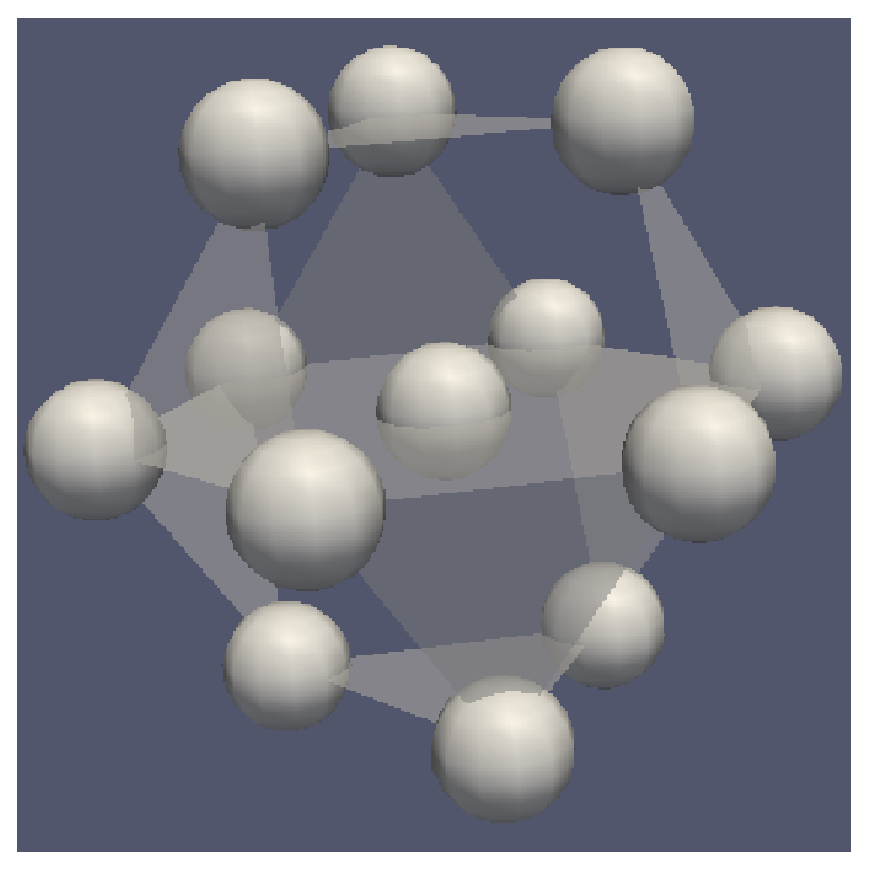
\includegraphics[width=0.27\textwidth]{fcc_13} & 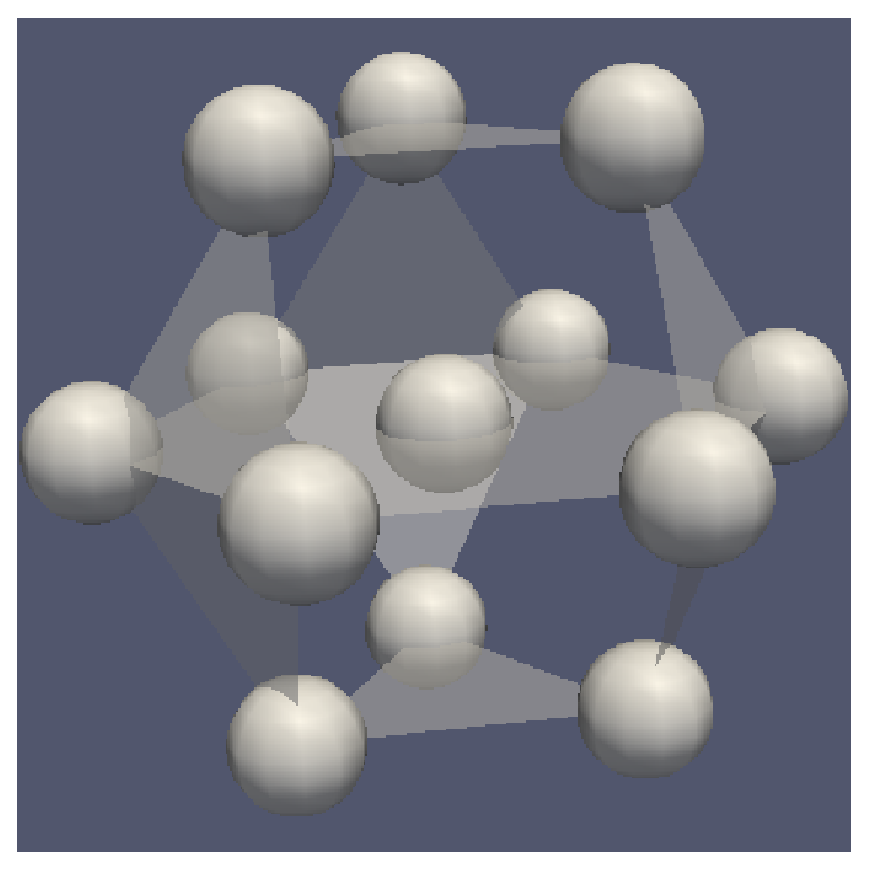
\includegraphics[width=0.27\textwidth]{hcp_13} & 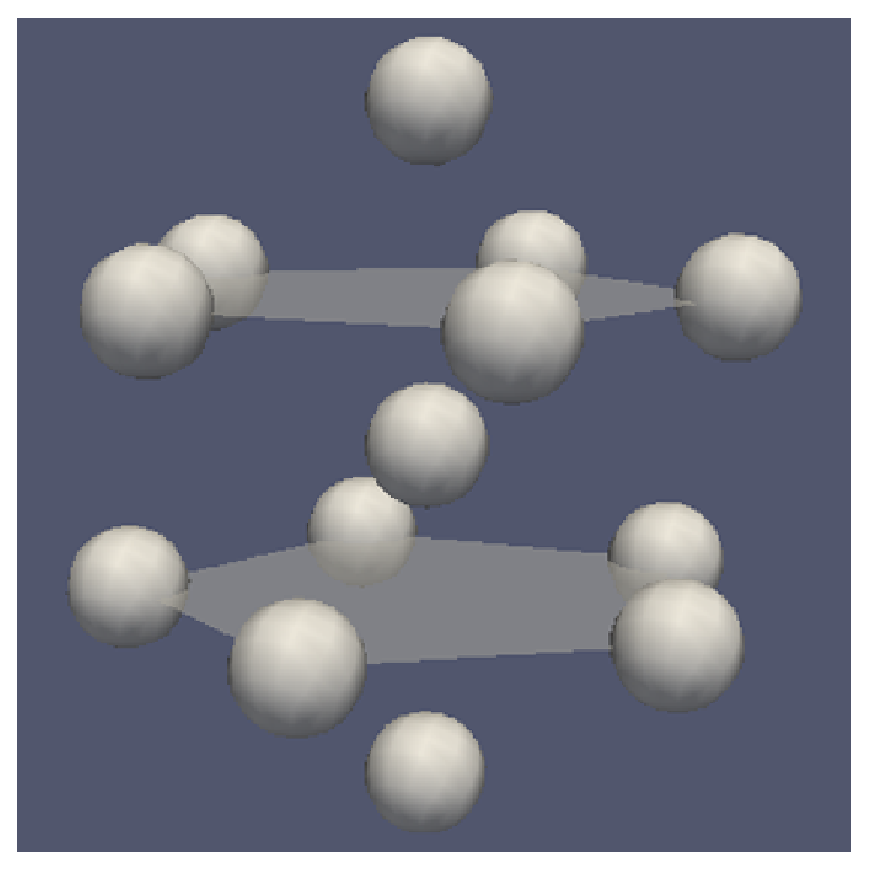
\includegraphics[width=0.27\textwidth]{ico_13}
	\end{tabular}
	\only<all:1>{\begin{tabular}{ccc}
	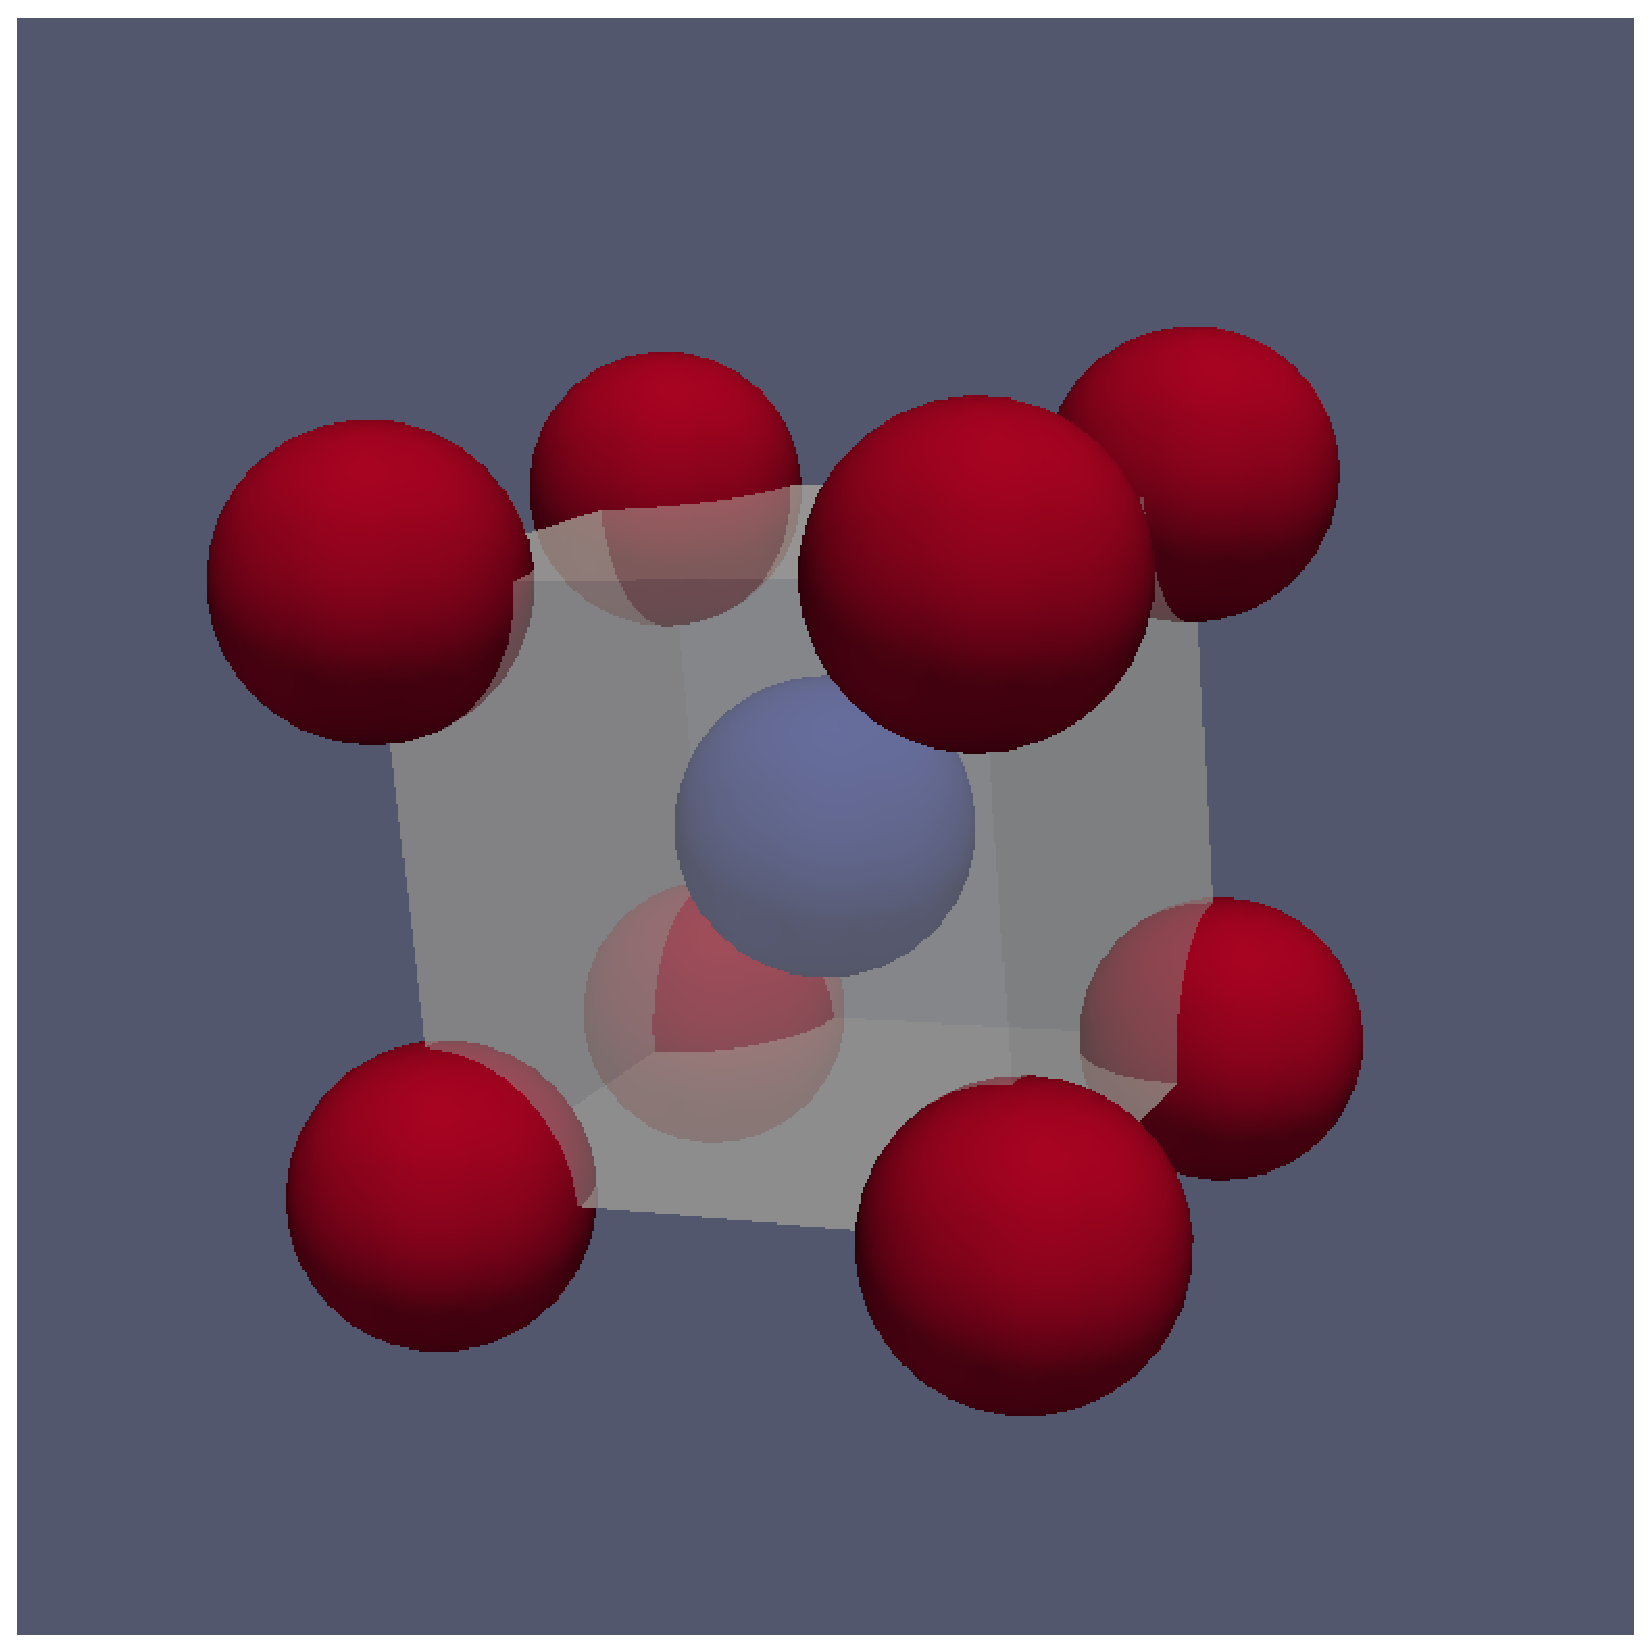
\includegraphics[width=0.27\textwidth]{bcc_9} & 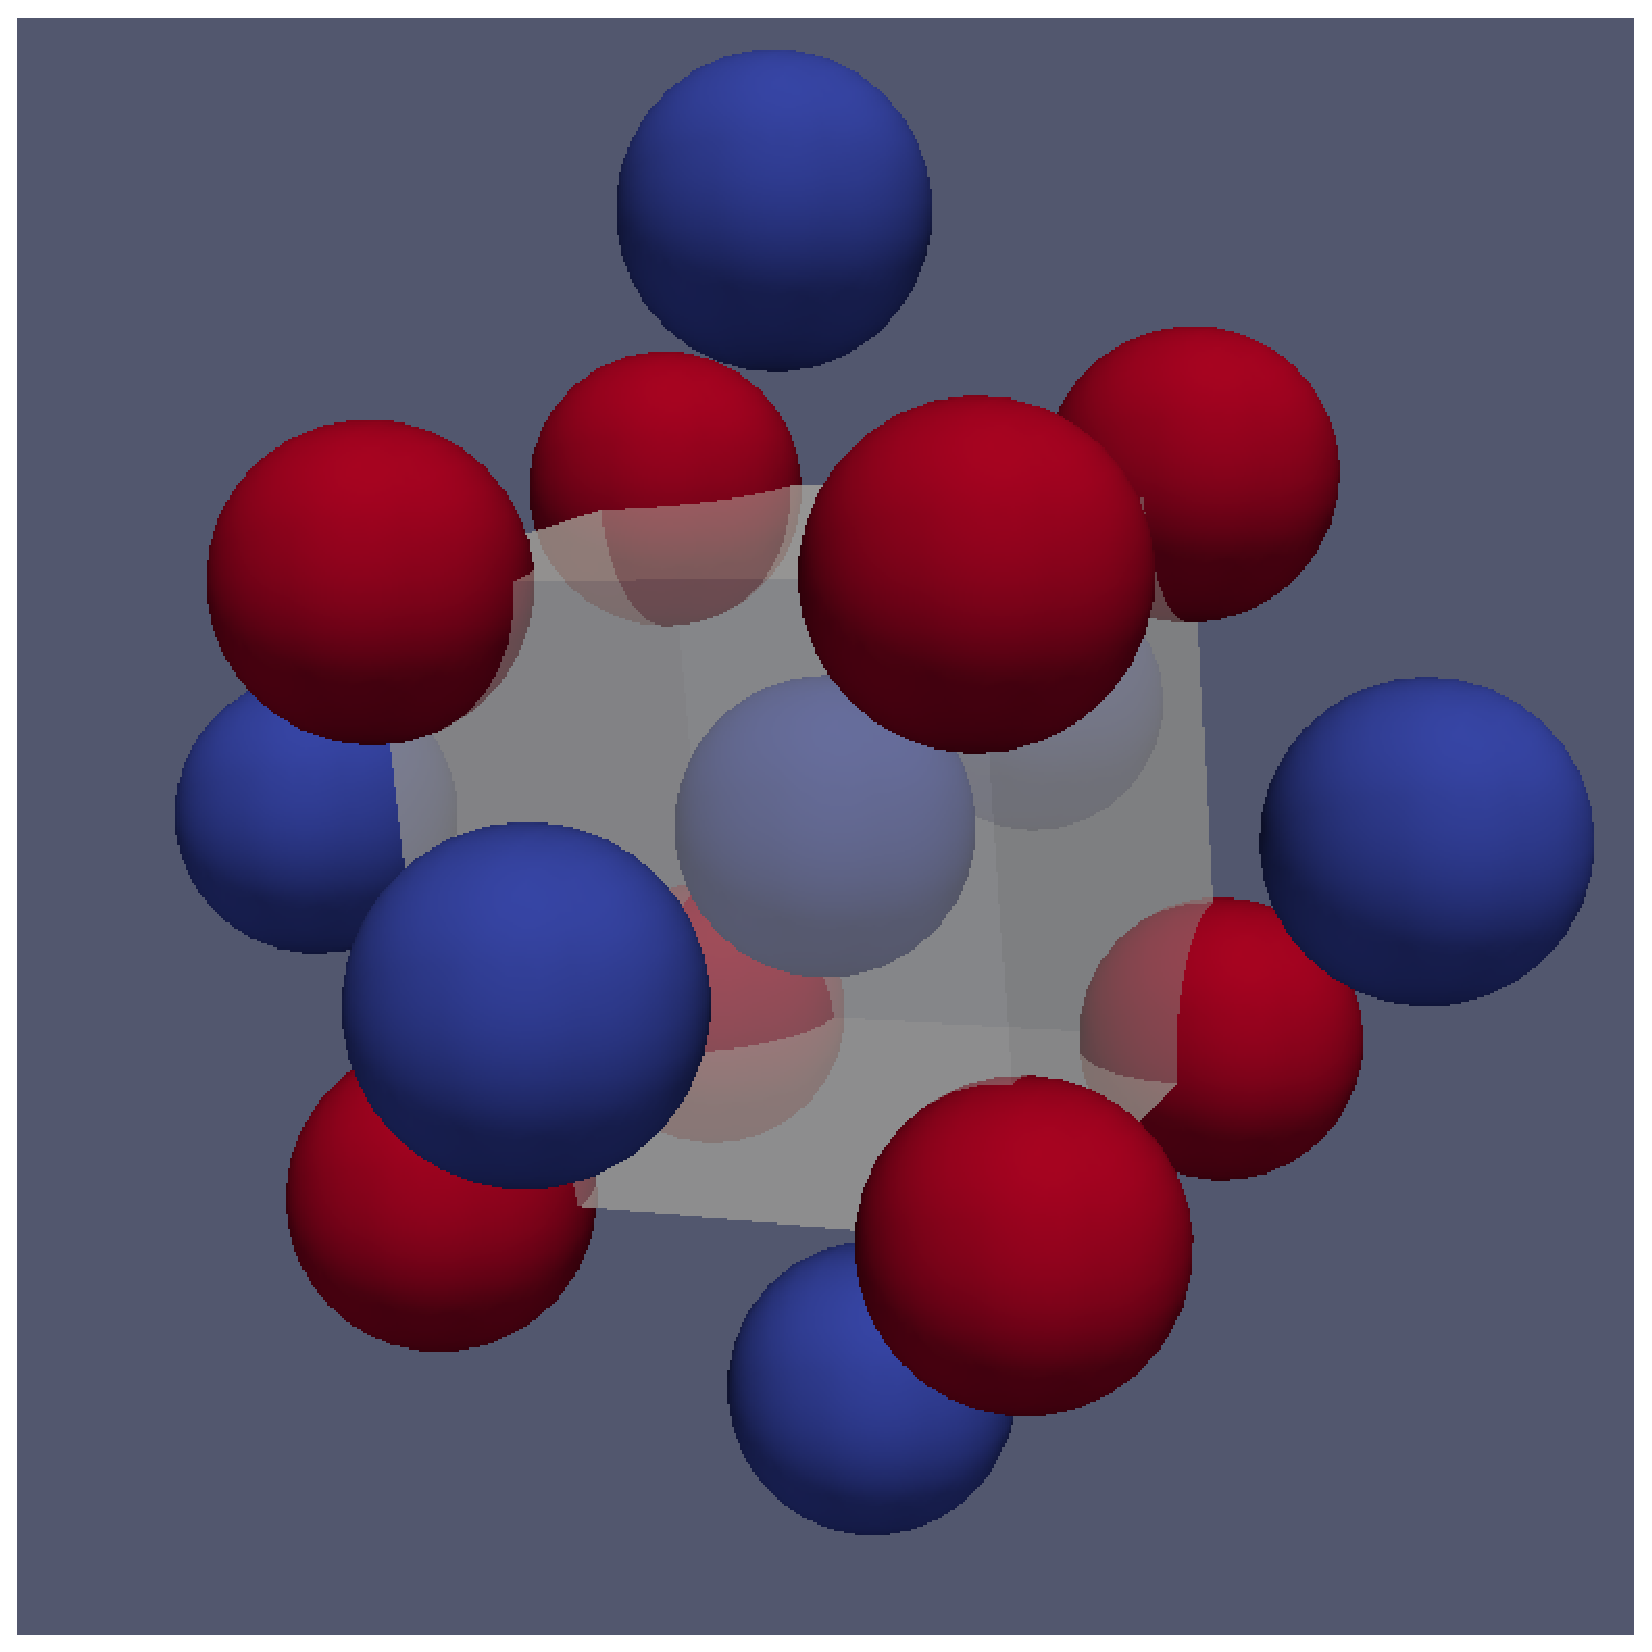
\includegraphics[width=0.27\textwidth]{bcc_15} & 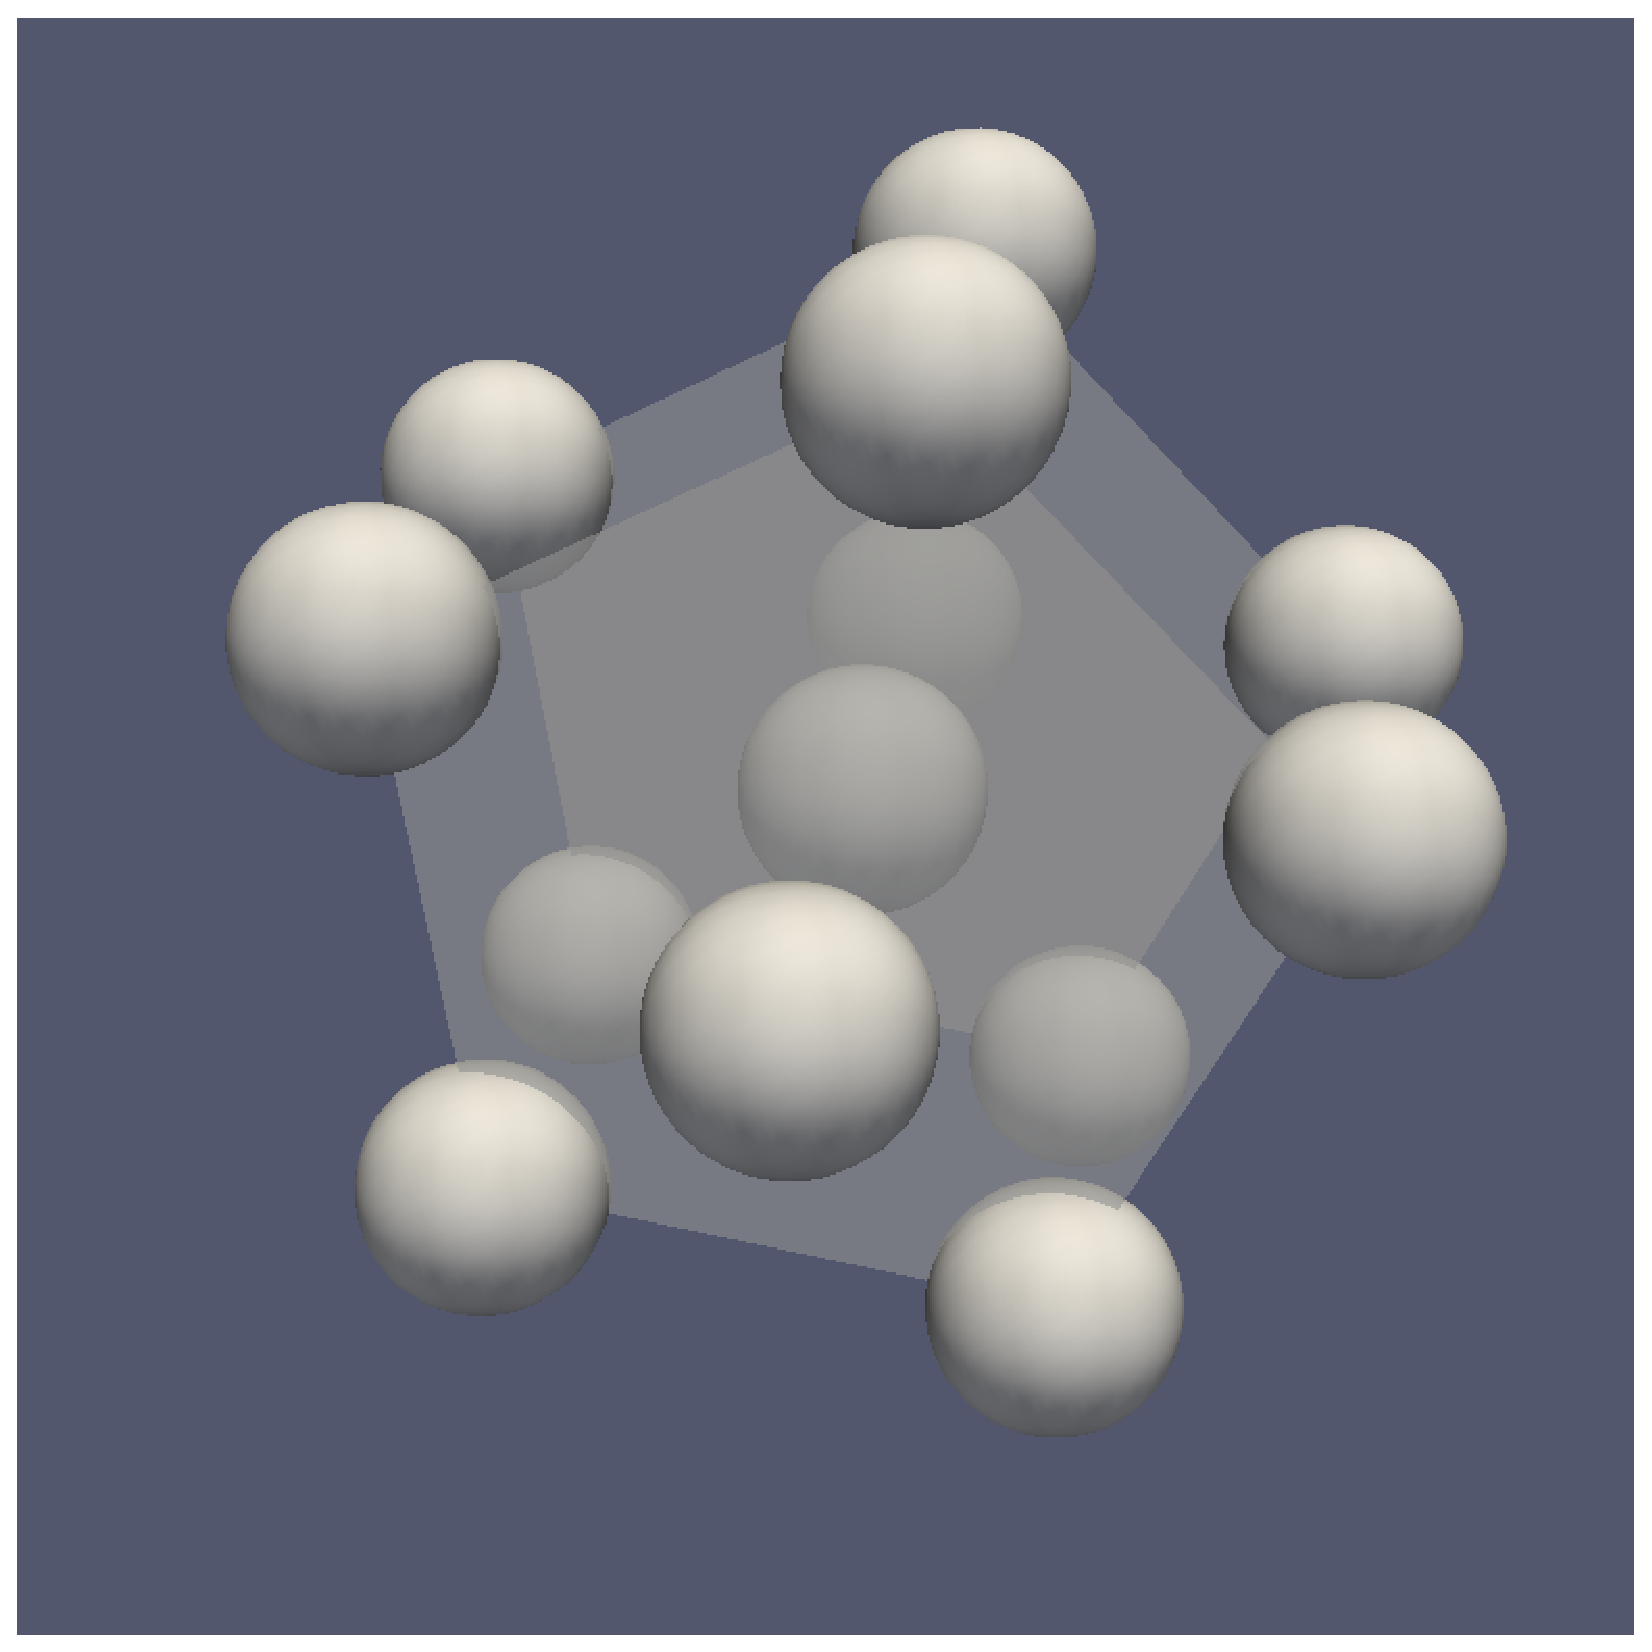
\includegraphics[width=0.27\textwidth]{dodec_13} \\ 
	\textsc{bcc} 9 & \textsc{bcc} 15 & Dodecahedron \\ 
	\end{tabular}}%
	\end{center}
	\only<all:2>{%
	\begin{itemize}
		\item The best ways to pack particles
		\item In hard spheres
		\begin{itemize}
			\item no potential energy
			\item ordering maximizes local vibrations
			\item vibrational entropy $\Leftrightarrow$ configurational entropy
			\item packing drives ordering
		\end{itemize}
	\end{itemize}
	
	\bigskip}%
\end{frame}

\subsection{Bond network}

\begin{frame}{Bond network - Neighbours}
	\begin{columns}
	\column{0.4\textwidth}
	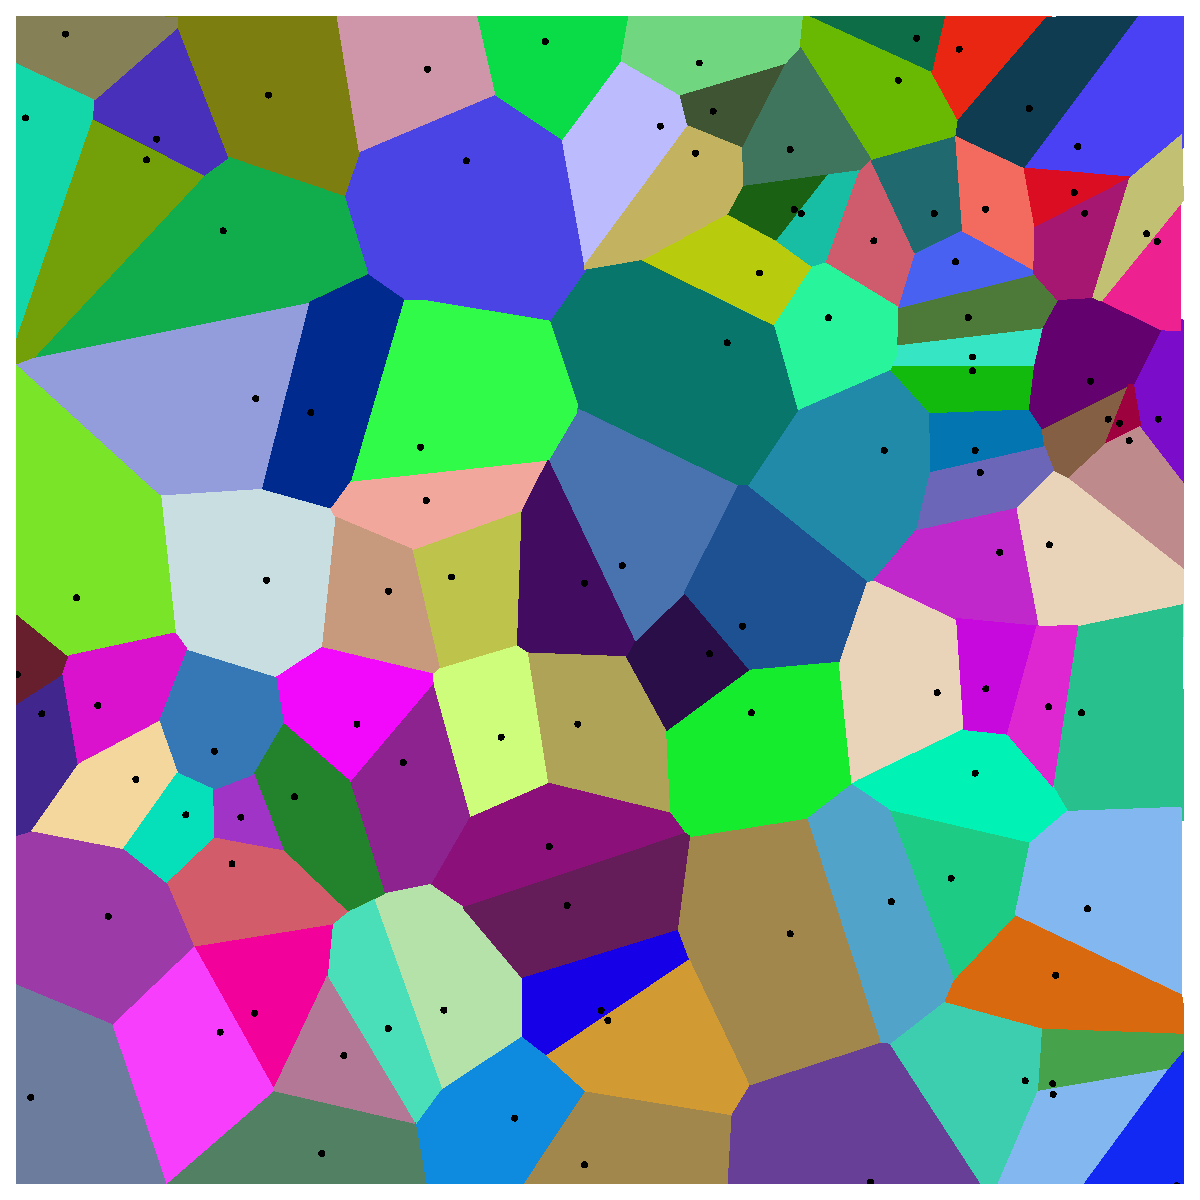
\includegraphics[width=\columnwidth]{voro2d}\\
	\centering Voronoi decomposition
	\column{0.6\textwidth}
	\centering Radial distribution function\\
	{\def\svgwidth{\columnwidth}\input{typicalRdf.pdf_tex}}
	\begin{itemize}
		\item A bond between neighbours
		\item Voronoi is not good (anisotropy)
		\item First shell
	\end{itemize}
	\end{columns}
\end{frame}

\begin{frame}{Topology of the bond network}
	\begin{columns}
	\column{0.25\textwidth}
	\centering \textsc{fcc}\\
	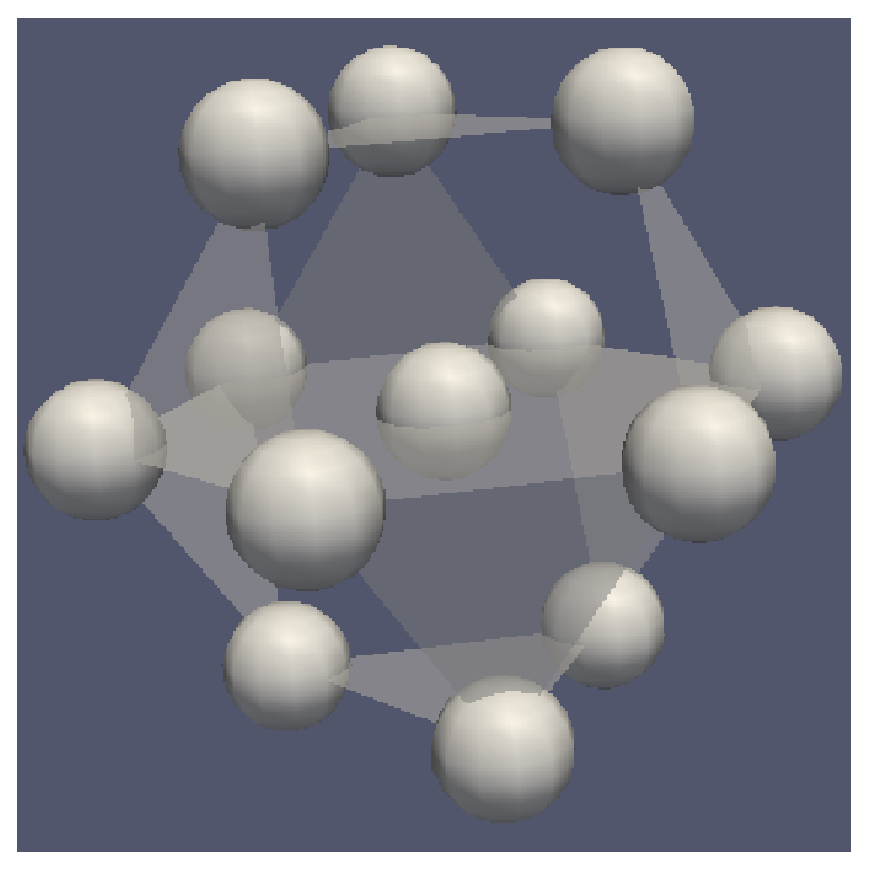
\includegraphics[width=\columnwidth]{fcc_13}
	
	\bigskip
	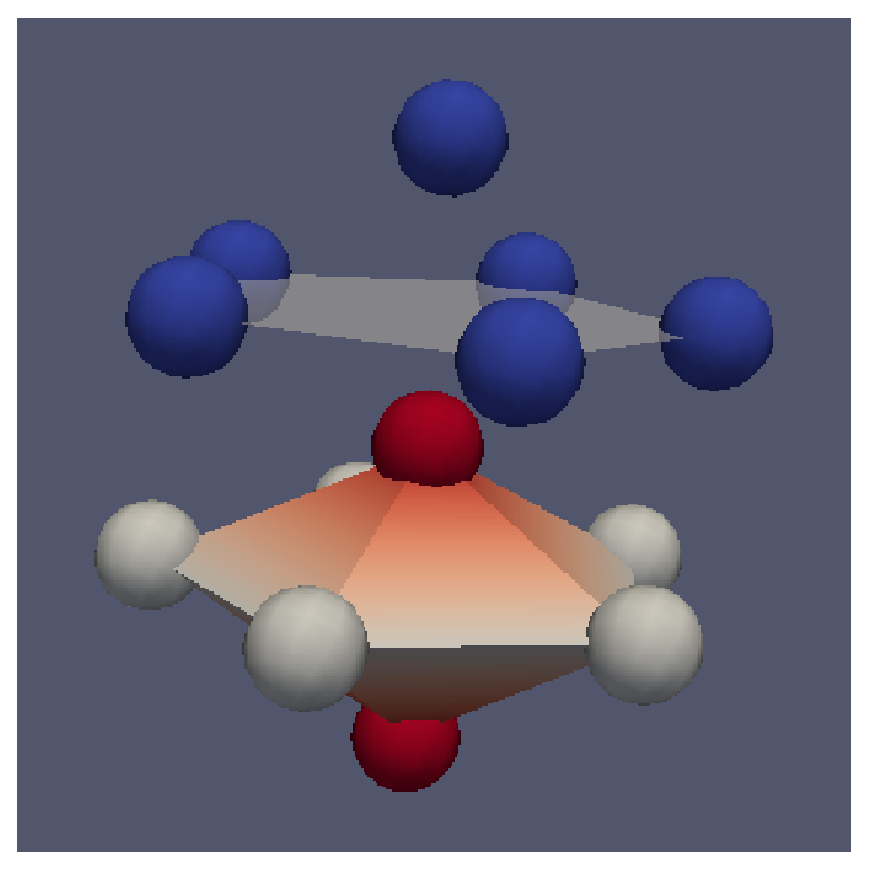
\includegraphics[width=\columnwidth]{ico_13_1551}\\
	Icosahedron
	\column{0.7\textwidth}
	\begin{itemize}
		\item Number of neighbours
		\item Voronoi signature \citet{tanemura1977geometrical}
		\item Common neighbours \citet{Honeycutt1987}
		\item Topological cluster classification \citet{Williams2007}
	\end{itemize}
	Difficult to correlate discrete categories in time or space.
	\end{columns}
\end{frame}

\subsection{Spherical harmonics}

\begin{frame}{Spherical harmonics}
	\begin{columns}
	\column{0.5\textwidth}
	\begin{itemize}
		\item Analogue to Fourier decomposition
		\item On a sphere
	\end{itemize}
	\column{0.5\textwidth}
	\[ h(\theta,\phi) = \sum_{\ell=0}^{\infty} \sum_{m=-\ell}^{\ell} q_{\ell m} Y_{\ell m}(\theta,\phi) \]
	\end{columns}
	\begin{description}
		\item[$\ell$] Order of symmetry
		\item[$m$] Orientation
		\item[$(r,\theta,\phi)$] Spherical coordinates
	\end{description}
	\begin{center}Altitude on earth: Decomposition\end{center}
	\begin{tabular}{ccc}
	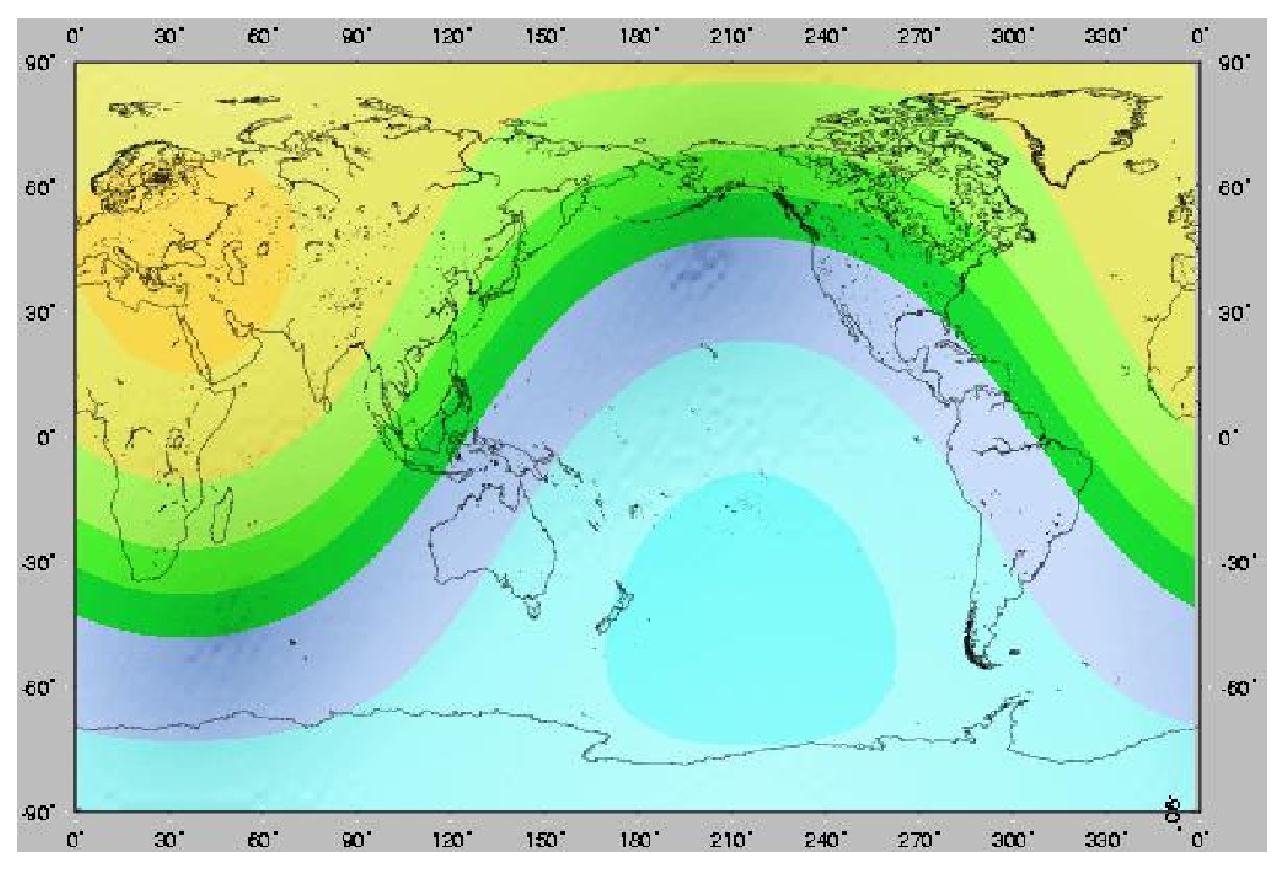
\includegraphics[width=0.29\textwidth]{earth_l1} & 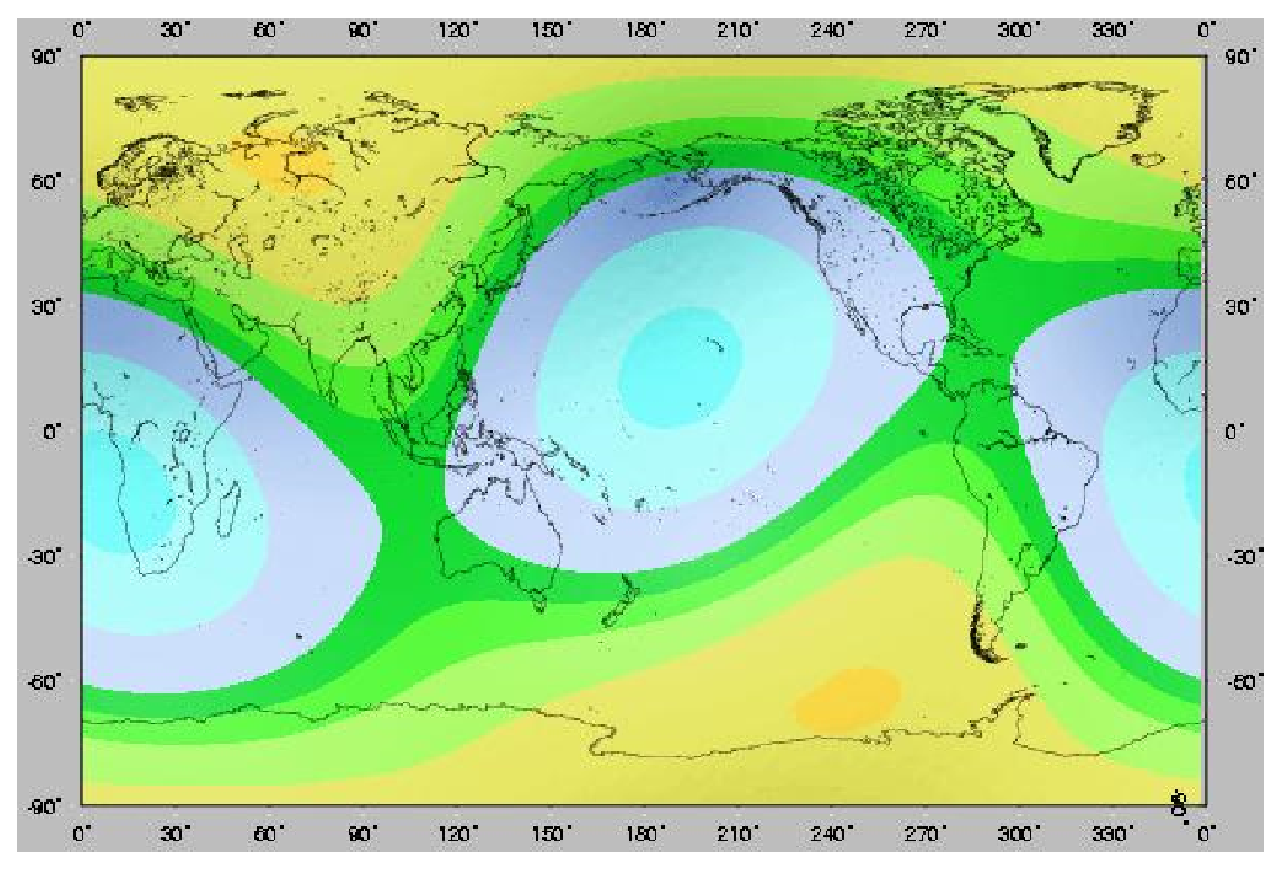
\includegraphics[width=0.29\textwidth]{earth_l2} & 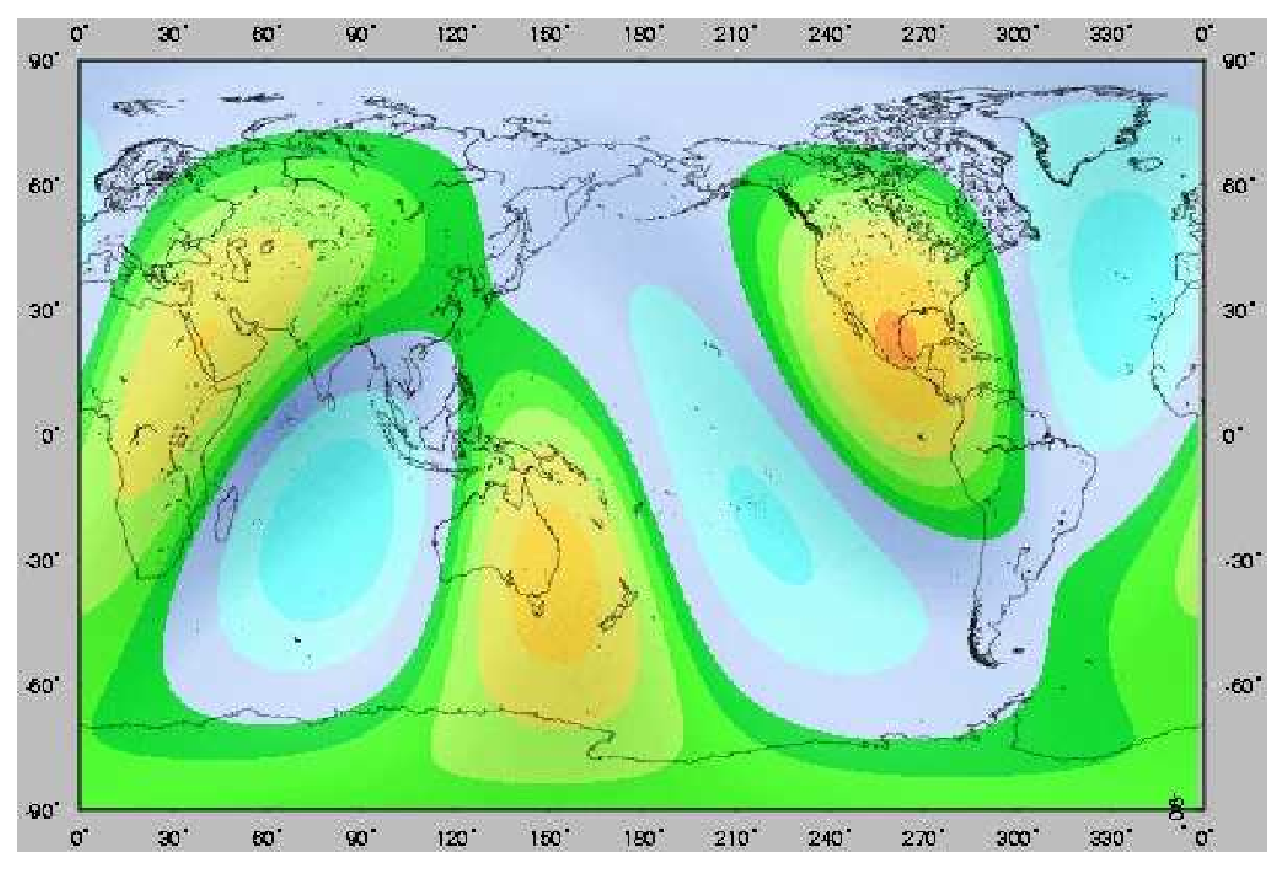
\includegraphics[width=0.29\textwidth]{earth_l3} \\ 
	$\ell=1$ & $\ell=2$ & $\ell=3$ \\ 
	\end{tabular} 
\end{frame}

\begin{frame}{Approximation by spherical harmonics}
	\begin{columns}[T]
	\centering
	\column{0.4\textwidth}
	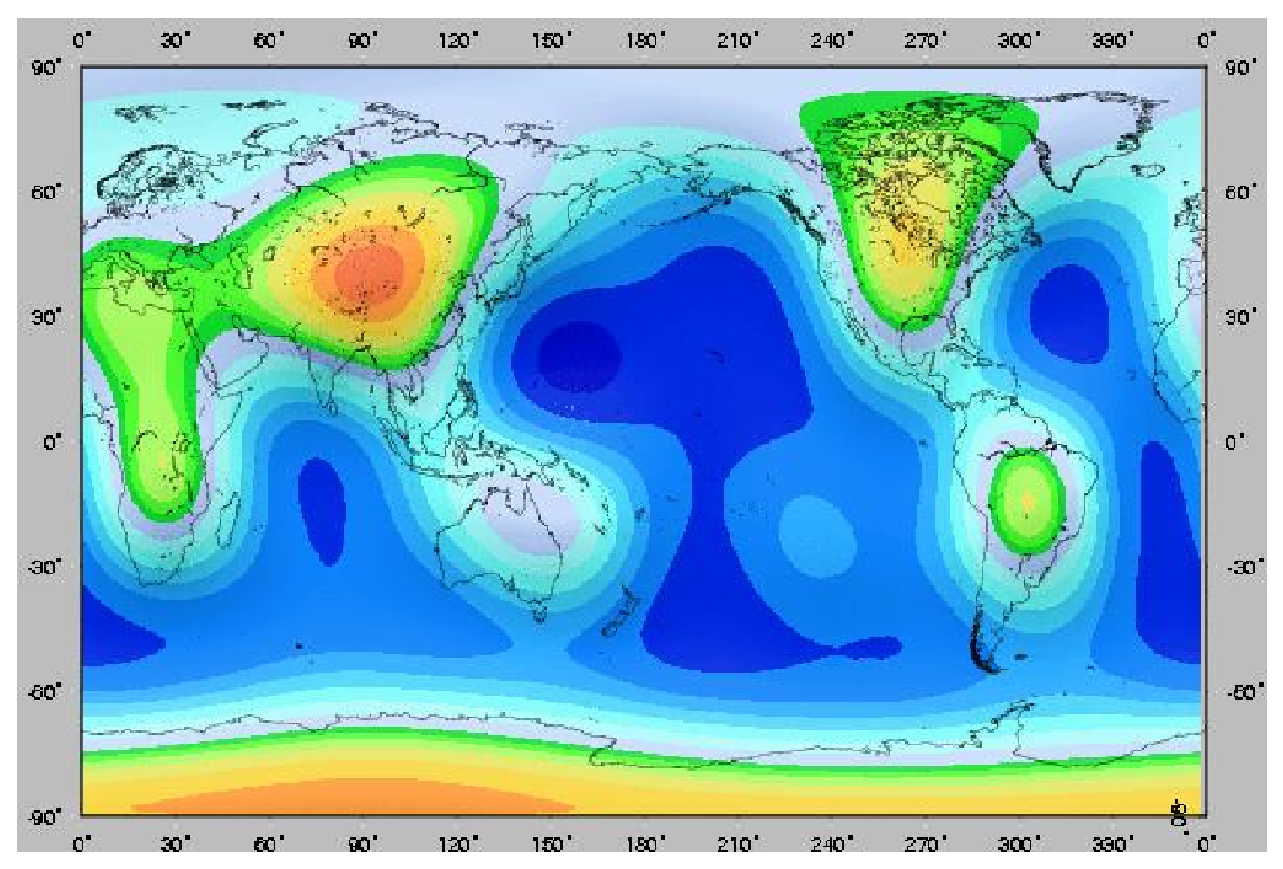
\includegraphics[width=\textwidth]{earth_to6}\\
	\centering{$\sum_{\ell=0}^6$}
	
	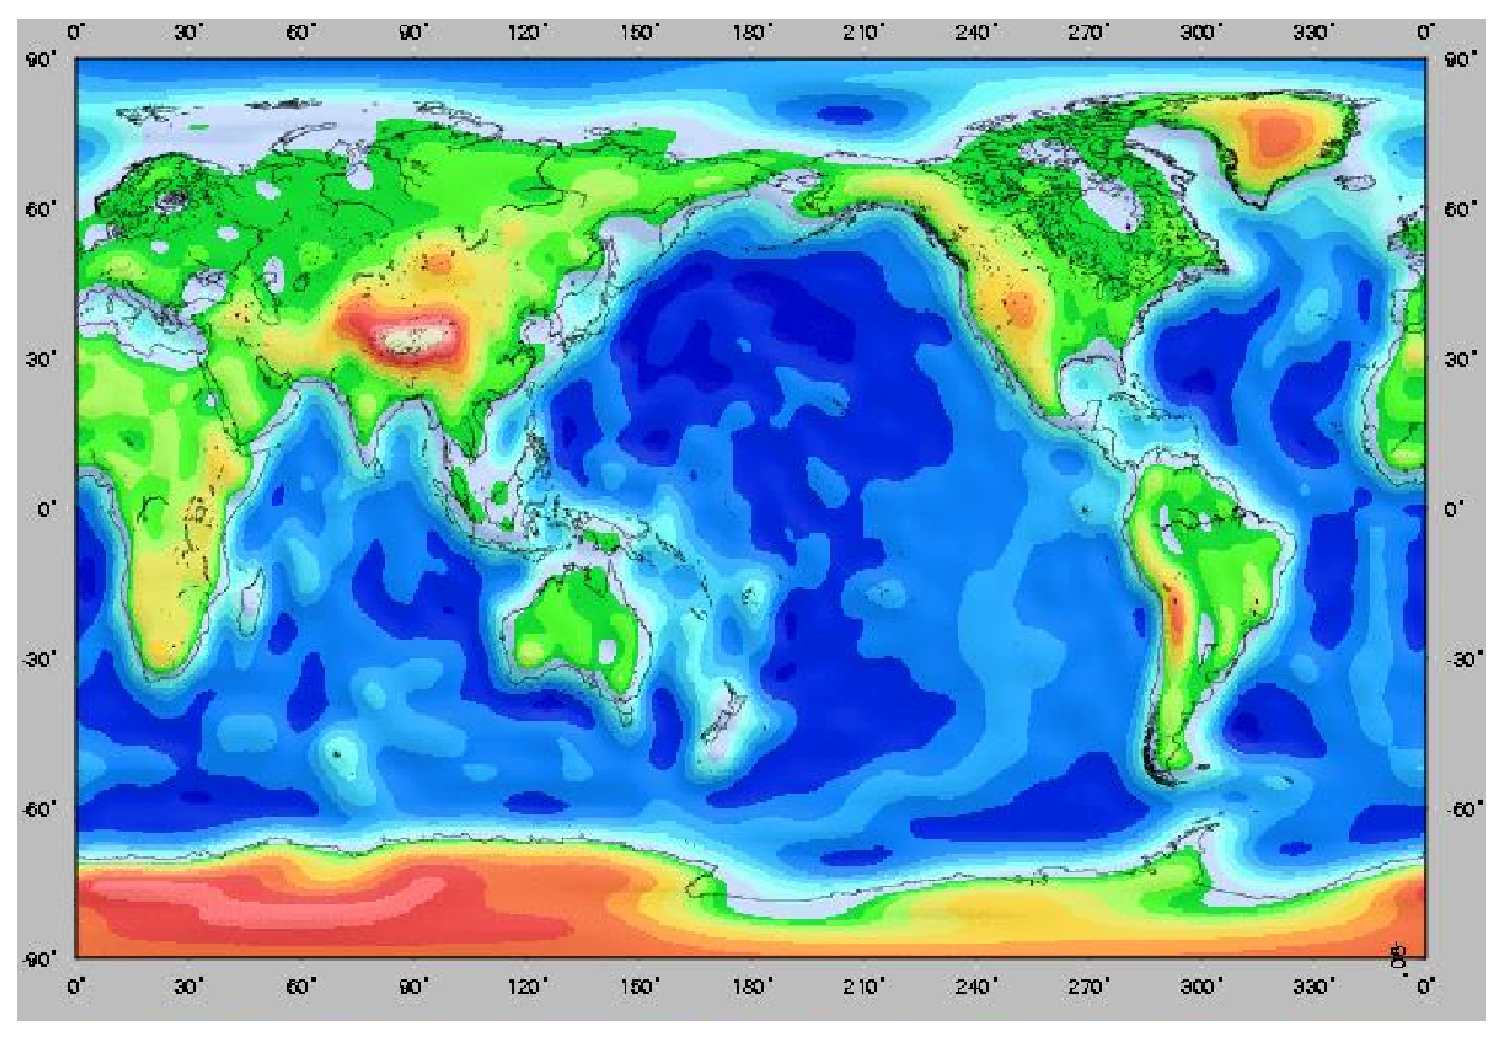
\includegraphics[width=\textwidth]{earth_to36}\\
	\centering{$\sum_{\ell=0}^{36}$}
	\column{0.4\textwidth}
	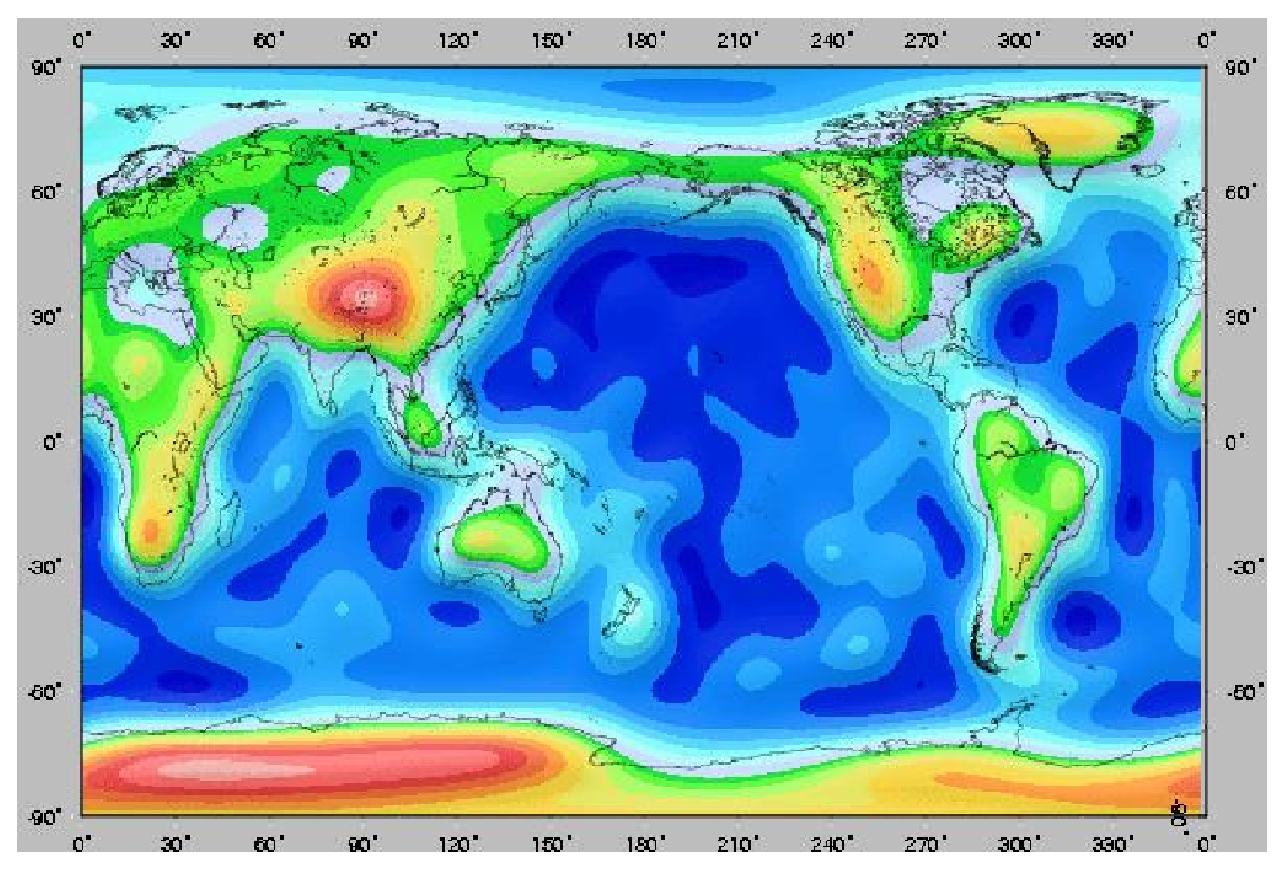
\includegraphics[width=\textwidth]{earth_to16}\\
	\centering{$\sum_{\ell=0}^{16}$}
	
	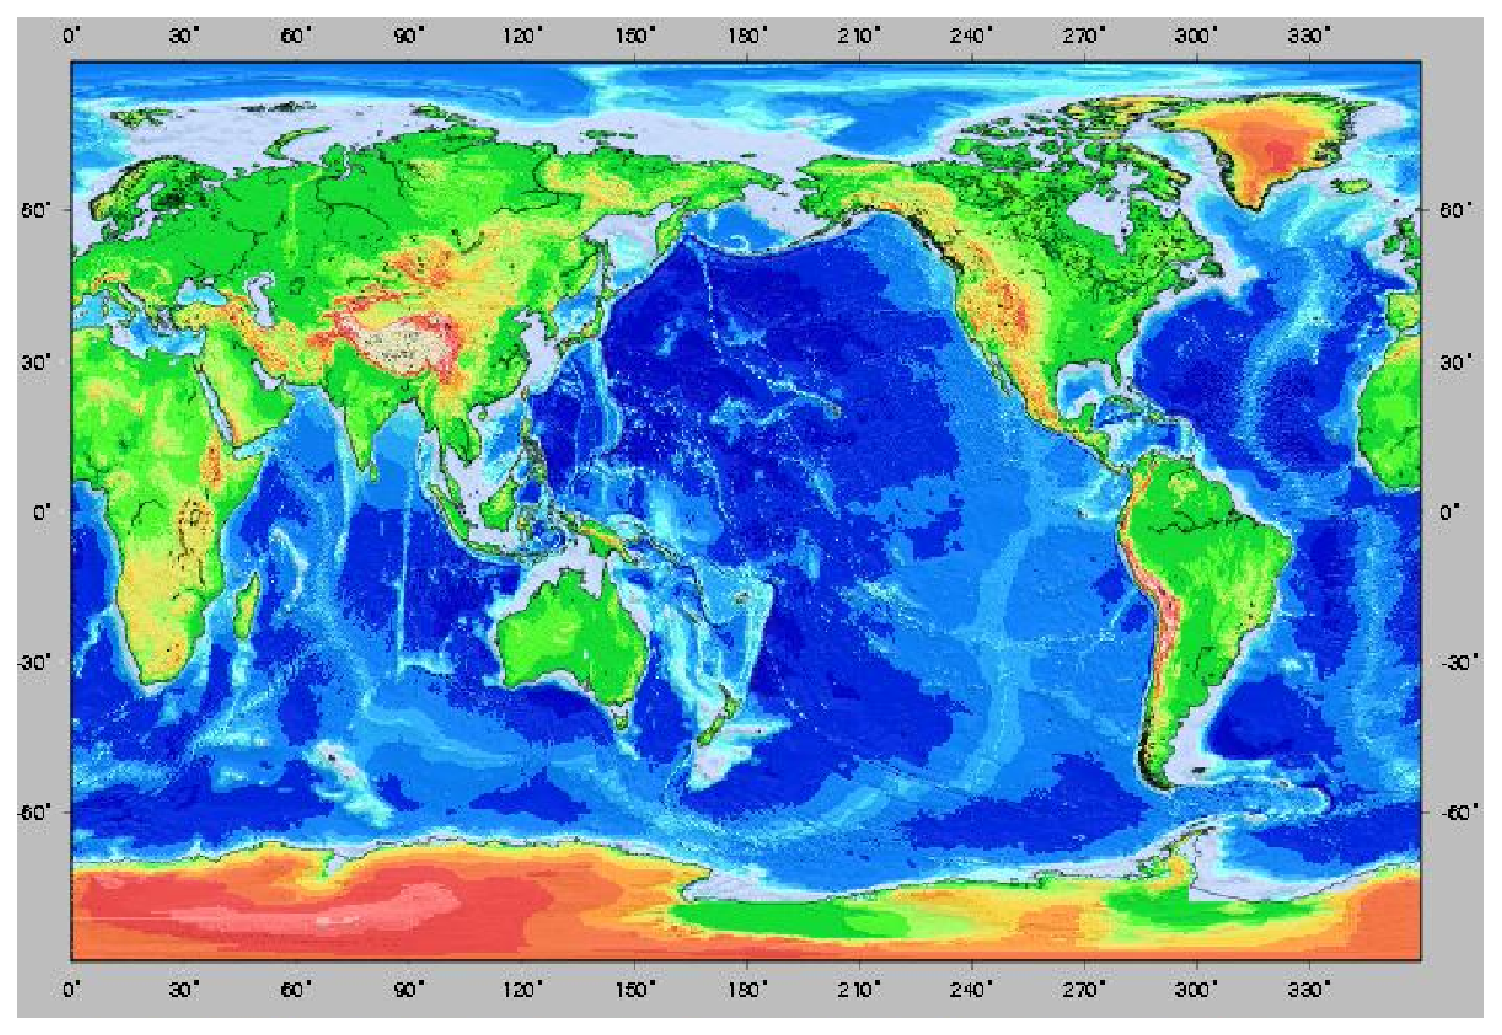
\includegraphics[width=\textwidth]{earth_grid}\\
	\footnotesize{Full grid of earth topography}
	\end{columns}
\end{frame}

\subsection{Bond orientational order}

\tikzsetnextfilename{spherical_harmonics_bis}
\againframe{local_sym_sh}

\begin{frame}{Bond orientational order}
	\begin{columns}
	\column{0.5\textwidth}
	\begin{itemize}
		\item A set of spherical harmonics for each
		\begin{itemize}
			\item Bond $\vec{r}_{ij}$
			\item Neighbourhood
		\end{itemize}
		\item Rotational invariants
		\begin{itemize}
			\item Strength of the $\ell$-fold symmetry
			\item Characterise the symmetry group
		\end{itemize}
	\end{itemize}
	\column{0.5\textwidth}
	\[ q_{\ell m}(i) = \frac{1}{N_i}\sum_{j=0}^{N_i} Y_{\ell m}(\theta(\vec r_{ij}),\phi(\vec r_{ij})) \]
	\[ q_\ell = \sqrt{\frac{4\pi}{2l+1} \sum_{m=-\ell}^{\ell} |q_{\ell m}|^2 } \]
	\end{columns}
	\[w_\ell = \sum_{m_1+m_2+m_3=0} 
			\left( \begin{array}{ccc}
				\ell & \ell & \ell \\
				m_1 & m_2 & m_3 
			\end{array} \right)
			q_{\ell m_1} q_{\ell m_2} q_{\ell m_3}\]
	\[\hat{w}_\ell = w_\ell{\left( \sum_{m=-\ell}^{\ell} |q_{\ell m}|^2 \right)}^{-\frac{3}{2}}\]
	
	\footnotesize{\citet{steinhardt1983boo}}
\end{frame}

\begin{frame}{Invariants distributions}
	\begin{columns}
	\column{0.6\textwidth}
	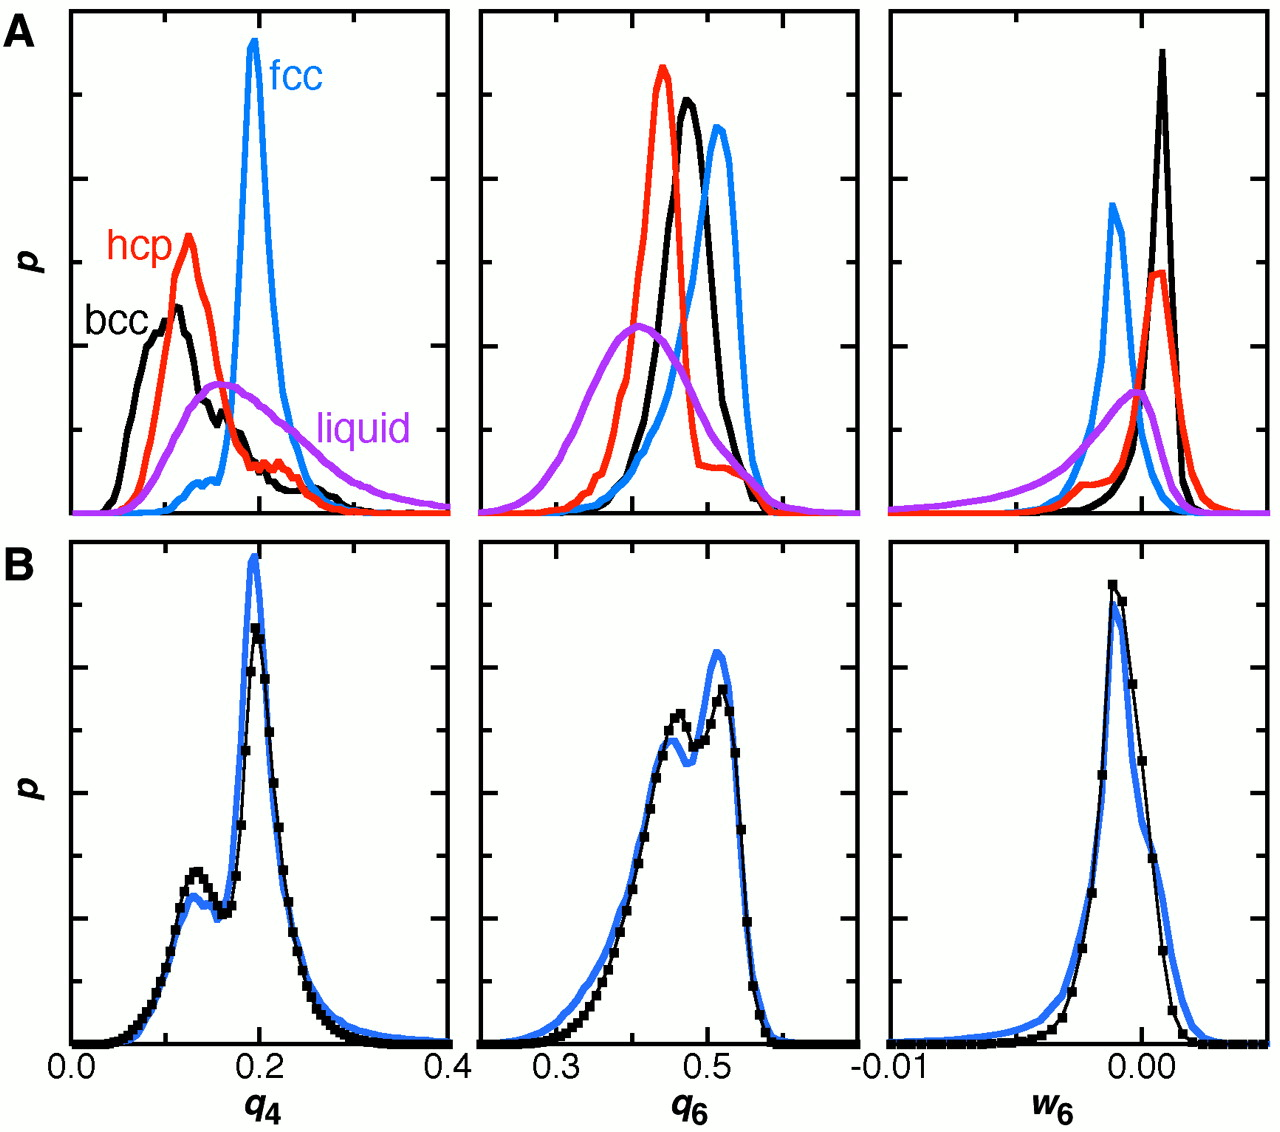
\includegraphics[width=\columnwidth]{gasser_invariants.jpg}
	\column{0.4\textwidth}
	\begin{itemize}
		\item Distributions are
		\begin{itemize}
			\item Noisy
			\item Broad
			\item Overlapping
		\end{itemize}
		\item Can characterize a sample
		\item Cannot characterize a single particle
	\end{itemize}
	\end{columns}
	\footnotesize{\citet{Gasser2001}}
\end{frame}

\begin{frame}{Coarse-grained BOO}
	\begin{columns}
	\column{0.6\textwidth}
	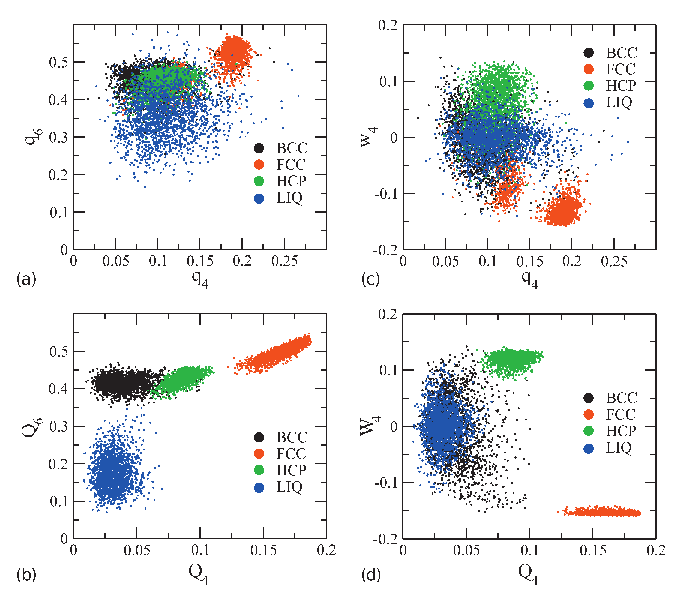
\includegraphics[width=\columnwidth]{invariants_maps_raster}
	\column{0.4\textwidth}
	\[ Q_{\ell m}(i) = \frac{1}{\tilde{N} (i)} \sum_{k=0}^{\tilde{N}(i)} q_{\ell m}(k) \]
	\begin{itemize}
		\item Take into account the second shell
		\item Structures with some periodicity are much better defined
		\item Non periodic structures goes to zeros
	\end{itemize}
	\end{columns}
	\footnotesize{\citet{lechner2008}}
\end{frame}

\begin{frame}{Crystal-like bond order}
	\begin{textblock*}{0.6\textwidth}(10mm,88mm)
		\simplephasediagram{\node at (0.576,0) [xp marker, fill=green!50!black] {};}
	\end{textblock*}
	\begin{columns}
	\column{0.7\textwidth}
	\tikzsetnextfilename{w4Q6}%
	\begin{tikzpicture}
		\pgfplotsset{
			extra tick style={grid=major},%
			every axis/.append style={%
				height=0.55\textwidth,
				ymin=0,ymax=0.6,%
				extra y ticks={\Qstar}, extra y tick labels={},%
				enlargelimits=false,axis on top,
				colormap={bw}{gray(0cm)=(1); gray(1cm)=(1); gray(10cm)=(0)},%
				colorbar sampled,%
				},%
		}
		\begin{groupplot}[
			group style={
				group size=2 by 1,%
				yticklabels at=edge left,%
				horizontal sep=0pt,%
				},%
			anchor=below south west,%
			width=0.55\columnwidth,%
			xtick scale label code/.code={},%
			colorbar horizontal, colorbar style={%
				samples=6, xtick={ 0.20,0.4,0.6, 0.8},% 
				extra y ticks={},%
				/pgfplots/colorbar shift/.style={yshift=0.3cm},
				at={(parent axis.north)}, anchor=below south, width=0.9*\pgfkeysvalueof{/pgfplots/parent axis width},
				xticklabel pos=upper,%
				label style={font=\footnotesize},
				},%
			]
		\nextgroupplot[%
			ylabel={$Q_6$}, xlabel=$Q_4$,%
			xmin=0,xmax=0.22,%
			colorbar style={%
				xlabel={per units of $Q_4\cdot Q_6$},% 
				xticklabels={$10^{1}$, $10^{2}$, $10^{3}$, $10^{4}$},%
				},%
			xticklabel={$\pgfmathprintnumber[fixed,precision=2]{\tick}$}
			]
		\addplot graphics
		[xmin=0,xmax=0.2,ymin=0,ymax=0.6]
		{Q4Q6go1};
		\node [below] at (axis cs:0.1909, 0.5745) {\textsc{fcc}};
		\node [below] at (axis cs:0.0972222, 0.484762) {\textsc{hcp}};
		\node [below] at (axis cs:0.0363696, 0.510688) {\textsc{bcc}};
		\draw[->, white,thick] (axis cs:0.05, 0.15) to [out=60, in=220] (axis cs:0.125, 0.4);
		
		\nextgroupplot[%
			xlabel=$10^3 \cdot w_4$, %
			xmin=-0.002,xmax=0.002,%
			xtickmin=-0.0015,%
			extra x ticks=0, extra x tick labels={},
			colorbar style={%
				xlabel={per units of $w_4\cdot Q_6$},% 
				xticklabels={$10^{3}$, $10^{4}$, $10^{5}$, $10^{6}$},%
				},%
			]
		\addplot graphics
		[xmin=-0.002,xmax=0.002,ymin=0,ymax=0.6]
		{w4Q6go1};
		\node [below] at (axis cs:-0.00067221, 0.5745) {\textsc{fcc}};
		\node [below] at (axis cs:7.47E-05, 0.484762) {\textsc{hcp}};
		\node [above] at (axis cs:0.0015, \Qstar) {\footnotesize{$Q_6^*$}};
		\draw[->, white,thick] (axis cs:0, 0.15) to [out=120, in=280] (axis cs:-0.0005, 0.4);
		\draw[->, white,thick] (axis cs:0, 0.15) to (axis cs:7E-05, 0.35);
		
		\end{groupplot}
	\end{tikzpicture}
	\column{0.3\textwidth}
	$w_\ell$ indicates how the $\ell$-fold symmetry is "rotating"

	\bigskip	
	
	\begin{itemize}
		\item No \textsc{bcc}
		\item Mainly \textsc{fcc}
		\item Some \textsc{hcp}
	\end{itemize}
	
	\bigskip
	
	We keep $Q_6$ as crystal axis
	\end{columns}
\end{frame}

\begin{frame}{Why $w_6$ and not $\hat{w}_6$}
\begin{columns}
\column{0.5\textwidth}
\resizebox{\columnwidth}{!}{\input{w6Q6quarter.pdf_tex}}
\column{0.5\textwidth}
\tikzsetnextfilename{hat_w6}
\begin{tikzpicture}
		\pgfplotsset{
			extra tick style={grid=major},%
			every axis/.append style={%
				height=0.8\columnwidth,
				ymin=0,ymax=0.6,%
				extra y ticks={\Qstar}, extra y tick labels={},%
				enlargelimits=false,axis on top,
				colormap={bw}{gray(0cm)=(1); gray(1cm)=(1); gray(10cm)=(0)},%
				colorbar sampled,%
				},%
		}
		\begin{axis}[
			anchor=above north west,%
			width=0.8\columnwidth,%
			xlabel=$10^2 \cdot w_6$,%
			xmin=-0.052,xmax=0.01,%
			extra x ticks={\wstar, -0.00782},%
			extra x tick labels={,},%
			xtick scale label code/.code={},%
			colorbar right, colorbar style={%
				samples=6, ytick={ 0.20,0.4,0.6, 0.8},% 
				yticklabels={$10^{1}$, $10^{2}$, $10^{3}$, $10^{4}$},%
				ylabel={per units of $w_6\cdot Q_6$},%
				extra x ticks={},%
				extra y ticks={},%
				label style={font=\footnotesize},
				},%
			]
		\addplot graphics
		[xmin=-0.052,xmax=0.052,ymin=0,ymax=0.6]
		{u6Q6go1_scale};
		\node at (axis cs:\wstar,0.6) (a) {};
		\node at (axis cs:-0.00782,0.6) (b) {};
		\node [below] at (axis cs:-0.0026, 0.5745) {\textsc{fcc}};
		\node [below, right] at (axis cs:-0.052, 0.05) {\textsc{Ico}};
		\draw[->, white,thick] (axis cs:-0.001, 0.15) to [out=90, in=275] (axis cs:-0.0015, 0.33);
		\draw[->, white,thick] (axis cs:-0.001, 0.15) to [out=180, in=30] (axis cs:-0.025, 0.12);
		\end{axis}
	\end{tikzpicture}
\end{columns}
\[\hat{w}_\ell = w_\ell{\left( \sum_{m=-\ell}^{\ell} |q_{\ell m}|^2 \right)}^{-\frac{3}{2}} \propto \frac{w_\ell}{q_\ell^3}\]
\end{frame}
%\tikzset{external/force remake}
\begin{frame}{Icosahedral network}
%\begin{figure}
	\centering
	\tikzsetnextfilename{percolation}%
	\begin{tikzpicture}[lab/.append style={below}]
	\pgfplotsset{ every axis/.append style={ width=0.4\textwidth, cycle list name=black white }}
	\pgfplotsset{cycle list name=black white}
	\begin{loglogaxis}[%
		xmin=10, xmax=1000, xlabel=\sffamily{Cluster size},%
		ymin=1, ylabel=\sffamily{Number of clusters},%
		]
		\addplot+[only marks] table {go1_w6_0012_sizes_rgs_noROI.hist};
		\addplot+[no marks, domain=50:500] {1e6*x^(-2.1)};
		\node[lab] at (rel axis cs:0.5, 0.95) {a};
	\end{loglogaxis}
	\begin{loglogaxis}[%
		at={(0.5\textwidth,0)},%
		xmin=10, xmax=1000, xlabel=\sffamily{Cluster size},%
		ymin=1, ylabel={$R_g/\sigma $},%
		ytick={1,10}, minor y tick num=10,%
		yticklabel={%
			\pgfmathfloatparsenumber{\tick}%
			\pgfmathfloatexp{\pgfmathresult}%
			\pgfmathprintnumber{\pgfmathresult}%
		},%
		]
		\addplot+[only marks] table[y expr=\thisrowno{2}/6.14] {go1_w6_0012_sizes_rgs_noROI.hist};
		\addplot+[no marks, domain=25:100] {0.75*x^(0.5)};
		\node[lab] at (rel axis cs:0.5, 0.95) {b};
	\end{loglogaxis}
	\begin{axis}[%
		at={(0, -0.3\textwidth)},%
		xlabel=$10^2 \cdot w_6$,%
		xmin=-0.03, xmax=0, xtick={-0.03, -0.02, -0.01}, xticklabels={$-3$, $-2$, $-1$}, minor x tick num=1,%
		xtick scale label code/.code={},%
		extra tick style={grid=major},%
		extra x ticks={\wstar, -0.00782},%
		extra x tick labels={,},%
		ymin=0,%
		ylabel=\sffamily{Largest cluster size},%
		]
		\addplot+[only marks] table {go1_w6.perco};
		\node [left] at (axis cs:\wstar,1e3) {\footnotesize $w_6^*$};
		\node [right] at (axis cs:-0.00782,1e3) {\footnotesize $w_6^\text{dod}$};
		\node[lab] at (rel axis cs:0.5, 0.95) {c};
	\end{axis}
	\begin{axis}[%
		at={(0.5\textwidth, -0.3\textwidth)},%
		xlabel=\sffamily{Fraction of activated particles},%
		xmin=0, xmax=0.6,ymin=0,%
		ylabel={Largest cluster size},%
		axis y line*=left,%
		]
		\addplot+[only marks] table [x index=2] {go1_w6.perco};
	\end{axis}
	\begin{axis}[%
		at={(0.5\textwidth, -0.3\textwidth)},%
		%xlabel={Fraction of activated particles},%
		xmin=0, xmax=0.6, ymin=0,%
		axis x line=none,%
		axis y line*=right, ytick=\empty,%
		ylabel=\sffamily{Percolation probability (a.u.)},%
		ylabel near ticks,%
		]
		\addplot+[only marks] coordinates{(1, 0)};
		\addplot[const plot, gray, fill=gray, semitransparent, area legend] file {go1_percol_thrs.hist};
		\node[lab] at (rel axis cs:0.5, 0.95) {d};
	\end{axis}
	\end{tikzpicture}
	%\caption{\textbf{Imperfect icosahedral clusters.} \textbf{a,} Cluster size distribution for nearly percolating threshold ($w_6<-0.012$). The exponent of random percolation ($-2.1$) is given by the straight line. 
%\textbf{b,} Radius of gyration (indicating a fractal dimension $d_f\approx 2$ given by the straight line) for the case of {\bf a}. \textbf{c,} Size of the largest non-percolating cluster as a function of the threshold on $w_6$. Percolation takes place near $w_6\approx -0.011$. Vertical lines indicate the position of $w_6^*$ and $w_6^\text{dod}$ respectively. \textbf{d,} Translation of \textbf{c} in terms of the fraction of activated particles (dots) together with the probability of the onset of percolation when particles are randomly activated (gray shading). We can see that activating particles as a function of icosahedral order and those activated randomly have almost the same percolation threshold ($\approx7.5\%$ of the particles activated).}
	%\label{fig:percolation}
%\end{figure}
\end{frame}

%\section{other parameters}


